\documentclass[12pt, a4paper]{article}
\setlength{\parindent}{0em}
\setlength{\parskip}{1.4ex}
\usepackage[english]{babel}
\usepackage[utf8]{inputenc}
\usepackage{graphicx}
\usepackage{amsmath}
\usepackage{listings}
\usepackage{textcomp}
\usepackage{xcolor}
\usepackage{fancyhdr}
\usepackage{caption}
\definecolor{listinggray}{gray}{0.9}
\definecolor{lbcolor}{rgb}{0.9,0.9,0.9}
\definecolor{backcolour}{rgb}{0.95,0.95,0.92}
\lstdefinestyle{JavaStyle}{
    language=Java,      % choose the language of the code
    deletekeywords={new,public},
    keywords=[2]{HashMap,Map,SimpleDateFormat,String},
    keywords=[3]{getKmaxDevice,getKmaxWidget,getKmaxHist,init},
    basicstyle=\scriptsize\ttfamily,
    keywordstyle=\color[RGB]{69,97,189},
    keywordstyle=[2]{\color{cyan}},
    keywordstyle=[3]\color[RGB]{137,77,155},
    commentstyle=\itshape\color{green!60!black},
    moredelim=[l][\itshape\color{gray}]{//}, %<--- overrides line-comment style
    stringstyle=\color[RGB]{192,8,8},
    numberstyle=\itshape\color{yellow!50!black},
    backgroundcolor=\color{lbcolor},
    tabsize=4,
    %   rulecolor=,
    upquote=true,
    aboveskip={1.5\baselineskip},
    columns=fixed,
    showstringspaces=false,
    extendedchars=false,
    breaklines=true,
    prebreak = \raisebox{0ex}[0ex][0ex]{\ensuremath{\hookleftarrow}},
    frame=single,
    numbers=left,
    showtabs=false,
    showspaces=false,
    showstringspaces=false,
}
\graphicspath{ {Billeder/} }
\pagestyle{fancy}
\fancyhf{}
\rhead{}
\chead{\leftmark}
\lhead{}
\cfoot{\thepage}
\renewcommand{\headrulewidth}{0pt}
\renewcommand{\footrulewidth}{0pt}
\title{Alquerque}
\author{Danny Nicolai Larsen, Mikkel Brix Nielsen \& Steffen Bach}
\date{\today}
\begin{document}
\maketitle
\newpage
\tableofcontents
\newpage

\section{Introduction}

For phase 2 of the project, we have been tasked with implementing the two classes \emph{Board} and \emph{Move} for the board game, Alquerque, by developing two classes in accordance with the contract for phase 2. The new \emph{Board} and new \emph{Move} class must be compatible with the previously developed Alquerque interfaces from phase 1. Furthermore, the \emph{Board} and \emph{Move} class must be developed as generally as possible to ensure its compatibility, not only with our interface, but also other interfaces developed in accordance with the contract for phase 1. The classes do not have to be executable, meaning neither of them have a main method. Testing the classes thus requires that a separate executable main method is developed to test the functionality of the two classes independently and coherently. All the provider classes, except for the ones being developed in phase 2, are precompiled, and thus we shall focus on the classes for \emph{Board} and \emph{Move} during this phase.

\section{Design choices}

\subsection{\emph{Move}}
To keep the class simple and easily understandable, the class \emph{Move} was developed with two attributes, int \emph{from} and int \emph{to}, which keep track of where from the move should start and where to the move should end, respectively.
These attributes have been made private, as it should not be possible to change a move once it has been made. Due to the nature of the private access modifier, these attributes are not accessible through \emph{object.attribute} syntax. For the \emph{Board} class to have access to where from and where to, a move should be made, respective getters for both attributes were made. There are no setters since the only time it should be possible to set the value of from and to is when a new instance of \emph{Move} is created. 

\subsection{\emph{Board}}
The \emph{Board} class and its methods have been developed based on a char array. This class has six attributes, which include a char array \emph{board}, an int \emph{turn}, which keeps track of how many turns have been played, a boolean \emph{isWhite}, which keeps checks whether it is white’s turn, a boolean \emph{isGameDone}, which ensures that int \emph{finishedGames} can only be incremented once for each instance of \emph{Board}, a static int \emph{finishedGames}, which keeps track of how many games have been played, and a static final char (constant) \emph{EMPTY}, which is the character to represents empty cells on the board.

\subsubsection{\emph{Board()}}
The board's constructor contains no arguments and, when called, it creates a char array of length 26 in the game's starting position. Index 0 is empty and indices 1 through 12 are filled with black pieces, represented by a ‘B’, the 13th space is empty, and indices 14 through 25 are filled with white pieces, represented by a ‘W’. The turn being set to 1, \emph{isWhite} is set to be based upon what turn it is, and \emph{isGameDone} set to false. 

\subsubsection{\emph{black()} \& \emph{white()}}
There are two methods, \emph{black()} and \emph{white()}, which individually loop through the char array that represents the board, each returning an int-array containing all the positions corresponding to their respective pieces. This is done by checking whether a cell contains either a black piece, ‘B’, or a white piece, ‘W’, and adding their position to their respective array, through their respective methods.

\subsubsection{\emph{isLegal()}}
For \emph{isLegal()}, it is designed to go through every combination of characteristics that would cause a move to be illegal according to the rules of Alquerque. In other words, every move with a set of characteristics is prohibited, is filtered away, and so only a move that passes through this filter is considered legal.

\subsubsection{\emph{legalMoves()}}
For the design of \emph{legalMoves()}, it goes through all cells where a piece is located and checks if it can make a legal move to any of all the other cells. If it encounters a legal move it is added to an array of Move objects and returned. To make this a bit more effective, it skips moves that would start from an empty cell.

\section{Implementation \& functionality}

\subsection{The methods \emph{black()} \& \emph{white()}}
The implementation of the methods \emph{black()} and \emph{white()} are identical except the fact that \emph{white()} looks for white pieces and \emph{black()} looks for black pieces. The methods work by creating a \emph{new ArrayList$<$Integer$>$()} and using a for-loop to go through \emph{this.board} looking for a corresponding piece and adding its index to the respective created arraylist. Afterwards, the arraylist is converted to an integer-array with the size of the created arraylist. This is done by initializing \emph{int[] nameOfIntegerArray = new int[nameOfArrayList.size()]} before going through the created arraylist with a for-loop, making the index in the integer-array equal the index in the arraylist. The method then returns the integer-array containing all the positions of the white and black pieces, respectively.

\begin{lstlisting}[style=JavaStyle]
/**
* Returns the positions of all white pieces on the board.
* @return the positions of all white pieces on the board.
*/
public int[] white() {
ArrayList<Integer> whitePieces = new ArrayList<Integer>();
for (int i = 1; i <= 25; i++)
if (this.board[i] == 'W')
whitePieces.add(i);
int[] white = new int[whitePieces.size()];
for (int i = 0; i < whitePieces.size(); i++)
white[i] = whitePieces.get(i);
return white;
}
\end{lstlisting}

For black: ‘W’ would be replaced with ‘B’ and the variable names would be different, but the implementation is the same.

\subsection{The method \emph{isLegal()}}
The boolean method, \emph{isLegal()}, works by taking an instance of the class Move as an argument and checking whether it is legal according to the rules of Alquerque. A series of if- and else-if-statements filters away any move with a set of characteristics that would make it illegal, and so, whenever a move passes through, \emph{isLegal()} returns true. \par 
This “filter” is implemented by checking the following criteria: \par
The position returned by \emph{to()} must always be empty. \par 
The position returned by \emph{from()} must be a piece corresponding to whoever's turn it is. So whenever \emph{isWhite} is true, the \emph{from()} position must contain a ‘W’ and whenever \emph{isWhite} is false, the \emph{from()} position must contain ‘B’. Speaking of which; \emph{isWhite} is an instance variable with a boolean value that is used in the code as a replacement to continuously write “turn \% 2 == 1” / “...0”  to check whether it is white or black to move, and for the code to be more easily serviceable as well as improved code-readability. \par
The absolute difference in columns between \emph{from()} and to() must never be greater than 2. For this, we made the auxiliary method, fileDiff(). The method, fileDiff(), returns an int, calculated by subtracting 1 from the positional value returned by to() and \emph{from()}, respectively, modulo 5, and adding 1 back to both, before subtracting one from the other, and returning the absolute value thereof. \par 
The difference between the \emph{from()} position and the to() position must be within -4 and -6 for white and within 4 and 6 for black. For this, we made the auxiliary method, pieceDiff(), which works by subtracting the value of to() by the value of \emph{from()}. By defining the legal difference to be -4, -5, and -6 for white, we ensure that only moves in the correct directions are allowed. The same thing applies to black with 4, 5, and 6 as legal positional differences between to() and \emph{from()}. \par
Normal moves from even-numbered positions must always be to an odd-numbered position, according to the rules of the game. \par
Take-moves from odd-numbered positions must always have an absolute positional difference of either 2, 8, 10 or 12. \par
And lastly, take-moves from even-numbered positions must have an absolute positional difference of either 2 or 10. \par
If an instance of Move breaks none of the aforementioned criteria, thereby passing through the filter, \emph{isLegal()} recognizes it as a valid move, in accordance with the current state of the board, on which it was called, and returns true. \par
The auxiliary method, \emph{isTakeMove()}, checks whether a move is considered a take-move by returning true if the pieceDiff() is greater than 6 or less than 4, albeit only if the piece taken is an opponent's piece, which is checked with the average positional value of to() and \emph{from()}.

\subsubsection{\emph{legalMoves()}}
The method \emph{legalMoves()} is implemented using an arraylist, which is then converted to an integer-array. Firstly a new arraylist of type move, called legalList is created. Then a for-loop is used to go through all cells of this.board and if that cell is not empty, then calculate all legalMoves from that cell to any other cells using another for-loop and creating new instances of Move, where the outer for-loops iterator variable is used as the origin of the move and the inner for-loops iterator variable is used as the destination for an instance of Move. IsLegal() is then called with that instance of Move as its argument, and if isLegal() returns true, that instance of move is added to the arraylist, legalList. Afterwards, the arraylist,legalList, is converted to an integer-array, legalMove, with the size of legalList. This is done by initializing \emph{int[] legalMove = new int[legalList.size()]} before going through legalListt with a for-loop, making the index in the legalMove equal the index in legalList. The method then returns the integer-array, legalMoves, containing all the legalMoves.

\subsubsection{\emph{move()}}
The method \emph{move()} takes an instance of the \emph{Move} class as a parameter and updates the \emph{board} array accordingly with the \emph{from()} and \emph{to()} getters for that move, it then checks if the move is a take-move, using the auxiliary \emph{isTakeMove()} method, and if this is true, it calculates the average positional value between \emph{to()} and \emph{from()} and removes the piece at that cell.
After exiting or skipping the if-statement it increments the \emph{turn} counter, and updates the \emph{isWhite} variable. Finally it uses the method \emph{isGameOver()} to check if the game has ended, and if it has, it increments the \emph{finishedGames} variable, and then sets the \emph{isGameDone} variable to true.

\subsubsection{\emph{isGameOver()} \& \emph{finishedGames()}}
The methods \emph{isGameOver()} and \emph{finishedGames()} are implemented in such a way that \emph{isGameOver()} returns whether there are no pieces remaining in \emph{white()} or whether there are no pieces left in \emph{black()} or whether there are no moves left in \emph{legalMove()} to indicate when the game represented by this board is over. \par
The static method \emph{finishedGames()} was implemented with the same functionality as a getter for the static class variable \emph{finishedGames}, meaning that when \emph{finishedGames()} is called on the class, \emph{Board}, it returns the value of the attribute \emph{finishedGames}.

\subsubsection{\emph{copy()}}
The method \emph{copy()} is implemented such that it creates a new instance of \emph{Board}, from the constructor, \emph{Board()}, called \emph{newBoard}. The respective char at each position on the board is copied via a for-loop to \emph{newBoard}, so that the current game gamestate of \emph{newBoard} matches the original board. Afterwards, the instance variables \emph{turn}, \emph{isWhite}, and \emph{isGameDone} for \emph{newBoard} are changed to equal the value of the original boards \emph{turn}, \emph{isWhite}, and \emph{isGameDone}, respectively. Lastly, \emph{newBoard} is returned as a copy of the instance of \emph{Board}, which \emph{copy()} was called upon. \par

\subsubsection{\emph{equals()}}
The \emph{equals()} method was implemented due to \emph{copy()} being overwritten. Overwriting \emph{copy()} could, potentially, make the original \emph{equals()} method return false on two copies of the same board. Therefore, a new \emph{equals()} was implemented, which created a filter of tests that ensures that the compared object does not equal null, which would return false, and that checks whether the instance of \emph{board} and the other object have the same memory address, which would return true. The last part of the filter checks whether the other object is an instance of \emph{Board}, which, if it is not, returns false, otherwise, \emph{other} is typecast to be a \emph{Board} called \emph{otherBoard}. Thereafter, the contents of each cell on \emph{otherBoard} is compared to the same cell on the instance of \emph{board}, that \emph{equals()} was called upon, through a while-loop, which increments a counter once every time both cells contain the same character. The loop is stopped at any point where two compared cells do have identical contents, or when the counter equals the length of the char array board. Finally, \emph{equals()} returns whether: The counter is equal to the length of the char array AND both boards are on the same \emph{turn} AND \emph{isGameDone} has the same boolean value for both.

\newpage

\subsubsection{\emph{hashCode()}}
The \emph{hashCode()} method was implemented due to \emph{equals()} being overwritten. This method is implemented by returning an integer based on the values of the attributes on the instance of the \emph{Board} that it is called upon. The attributes used to create the hashcode are \emph{board} and \emph{turn}. Even though \emph{board} is a char array, it needs to be converted to an integer first. This is done by calling \emph{hashCode()} for char arrays on \emph{board}. In short; the method returns the sum of \emph{board.hashCode()} and \emph{turn} multiplied by 31.

\newpage

\section{Testing}

\subsection{Test-approach for \emph{isLegal()}}
To thoroughly test whether \emph{isLegal()} worked as desired, it was convenient to use a testclient and create specific scenarios on a board. The method, \emph{isLegal()}, works like a filter for moves that are not allowed to be made. By testing several different sets of characteristics for a move to see whether it was allowed or not, it could effectively be ensured that no illegal move would ever pass through this so-called filter. Theoretically, this means that all 625 combinations of moves have been checked, but in a generalized sense that took a fraction of the time that otherwise would have been required to ensure proper functionality.

\subsection{Test of \emph{legalMoves()}}
To test the method \emph{legalMoves}, we modified our MainTest class to print out the contents of the array while playing. This seemed as an effective way of testing two things at the same time. One: That it stores valid moves correctly in the array; and two: That \emph{isLegal} works properly, which calculates all the valid moves available without returning any invalid moves. \par
Below is a sample output of the console during these tests.

\begin{figure}[h]
	\centering
	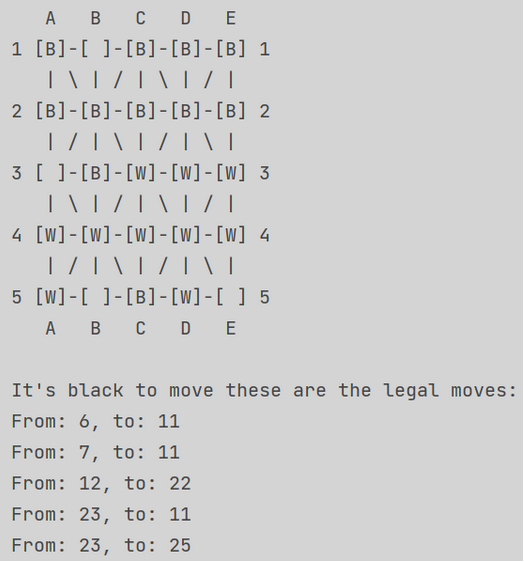
\includegraphics[width=0.5\textwidth]{isLegalprint.png}		
\end{figure}

\subsection{Sketchy take-moves}

The move from 19 to 13 would remove the piece on 16, regardless of color. \par

\begin{figure}[h]
	\centering
	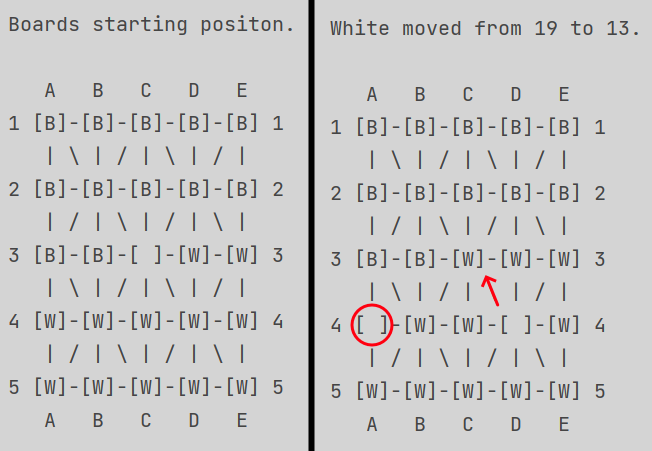
\includegraphics[width=0.7\textwidth]{19til13TakeFejl.png}	
\end{figure}

The same logic applied to the move 17 to 13, which would instead remove the piece on 15. 
Two things went wrong in these instances: Not only did white remove a white piece, it removed a piece whilst not being a take-move. \par So to kill two birds with one stone, we made the auxiliary boolean method, \emph{isTakeMove()}, to check whether the absolute positional difference between the value returned by \emph{from()} and the value returned by \emph{to()} was greater than 6 or less than 4, and to check whether the piece taken was an opponent piece. \par 
We later discovered certain cases where, as an example, a piece on 15 could take 16 and move to 17, which implied that more had to be done to check for the legality of a take-move. \par

\begin{figure}[h]
	\centering
	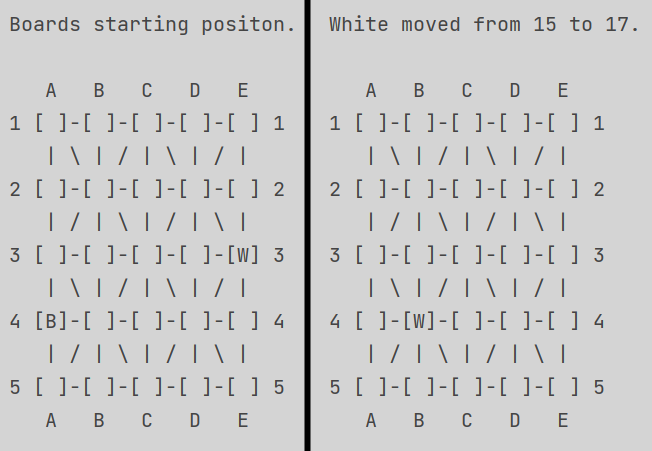
\includegraphics[width=0.7\textwidth]{15til17TakeFejl.png}	
\end{figure}

As the absolute positional difference of the move was 2, which is less than 4, and the piece on 16 was an opponent piece, it fully qualified for a legal take-move. \par To fix this as generally as possible, we made the auxiliary method, \emph{fileDiff()}, to check the difference between the from-file and the to-file. For a take-move to be legal, this would always have to be either 2 or 0. \par This method conveniently could have been used for non-take-moves as well, but that seemed redundant, as non-take-moves were only allowed to be within a specific range, which is a piece difference of min. 4, max. 6 for black and min. -6, max. -4 for white.

\subsection{Proof of \emph{isLegal()}’s functionality}
Below is a selection of examples of legal and illegal moves used to test the general functionality, which, as a result, should give sufficient confidence in the method, \emph{isLegal()}.

\begin{figure}[h]
	\centering
	\caption*{Moves in the right direction are valid moves}
	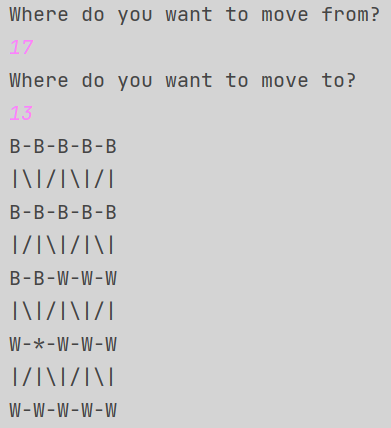
\includegraphics[width=0.4\textwidth]{isLegalProf/LovligeTrækOgTakeMoves/DuMåGodLaveLovligeTræk.png}	
\end{figure}

\begin{figure}[h]
	\centering
	\caption*{Moving pieces on the wrong turn are not valid moves}
	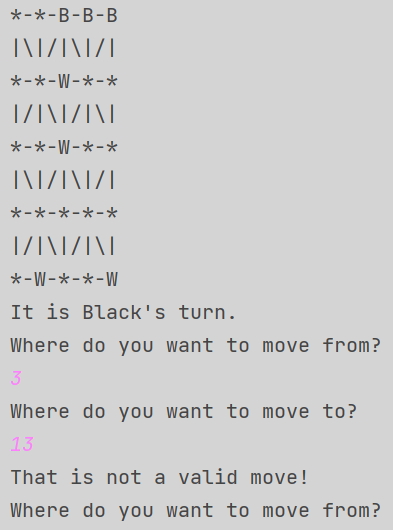
\includegraphics[width=0.4\textwidth]{isLegalProf/MåIkkeRykkeTilFelterDerStårEnBrik.png}	
\end{figure}

\begin{figure}[h]
	\centering
	\caption*{Take-moves in all directions are valid moves.}
	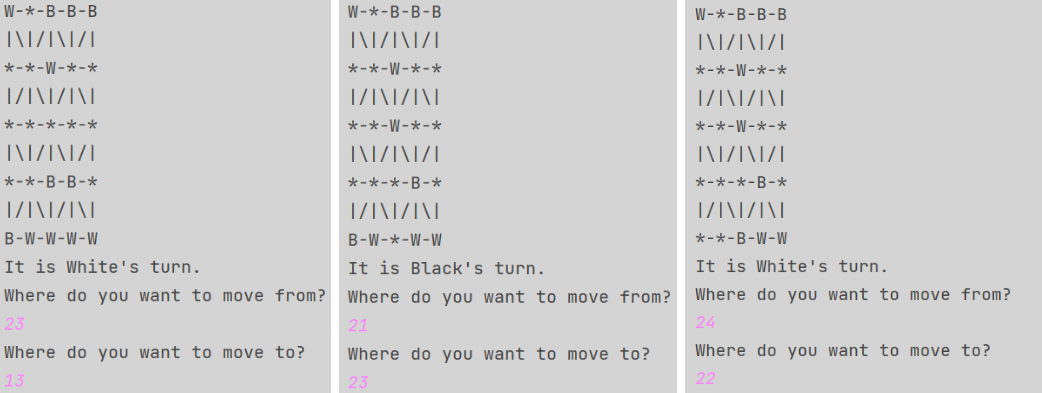
\includegraphics[width=1\textwidth]{isLegalProf/3in1.png}	
\end{figure}

\begin{figure}[h]
	\centering
	\caption*{Take-moves across the board are not allowed. Normal moves in a backwards direction are not valid moves.}
	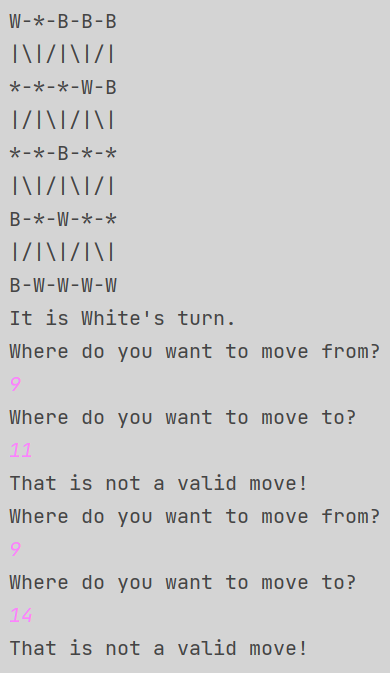
\includegraphics[width=0.4\textwidth]{isLegalProf/IkkeRykkeBagudEllerOutOfBounds.png}	
\end{figure}

\begin{figure}[h]
	\centering
	\caption*{Moves to a non-empty position are not allowed.}
	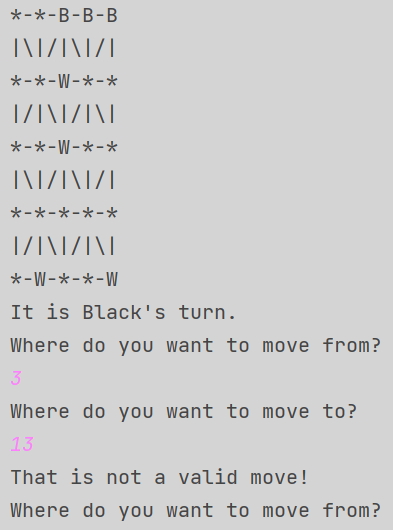
\includegraphics[width=0.4\textwidth]{isLegalProf/MåIkkeRykkeTilFelterDerStårEnBrik.png}	
\end{figure}
\clearpage
\subsection{Test of \emph{finishedGames()}} \par
To test \emph{finishedGames}, an impromptu client was made to initiate a game with ‘CPU vs. CPU’. After a game is finished, the user can choose to play again, which will initiate a new game. If the user chooses not to play again, the program will end. The \emph{finishedGames} attribute is incremented in \emph{move()} whenever \emph{isGameOver()} returns true. \par To check functionality, \emph{finishedGames()} was printed as “Games Played”, as seen on the image below. 
Note that the total number of wins, losses, and draws, which indicate the actual number of games played, does not match “Games Played” played when the next game is initiated. This is due to the fact that every copy of \emph{board} made by MiniMax, whenever an end-state is reached, also counts towards the total number of \emph{finishedGames}.

\begin{figure}[h]
	\centering
	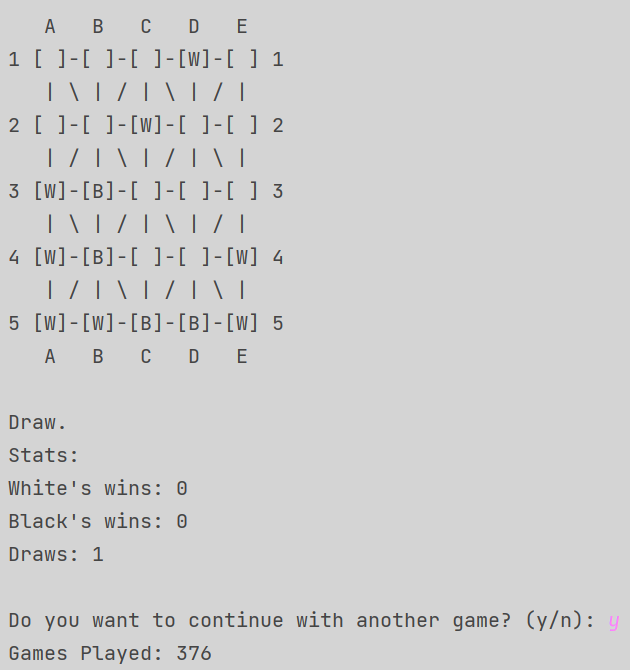
\includegraphics[width=0.6\textwidth]{TestAfFinishedGames.png}	
\end{figure}
\newpage
\subsection{Test of \emph{black()} \& \emph{white()}}
By printing the respective array of positions for black and white pieces, we ensure that \emph{black()} and \emph{white()} work as intended, which is that they return an array with the correct positions of their respective pieces on the board. Two of the tested board positions can be seen in the images below.

\begin{figure}[h]
	\centering
	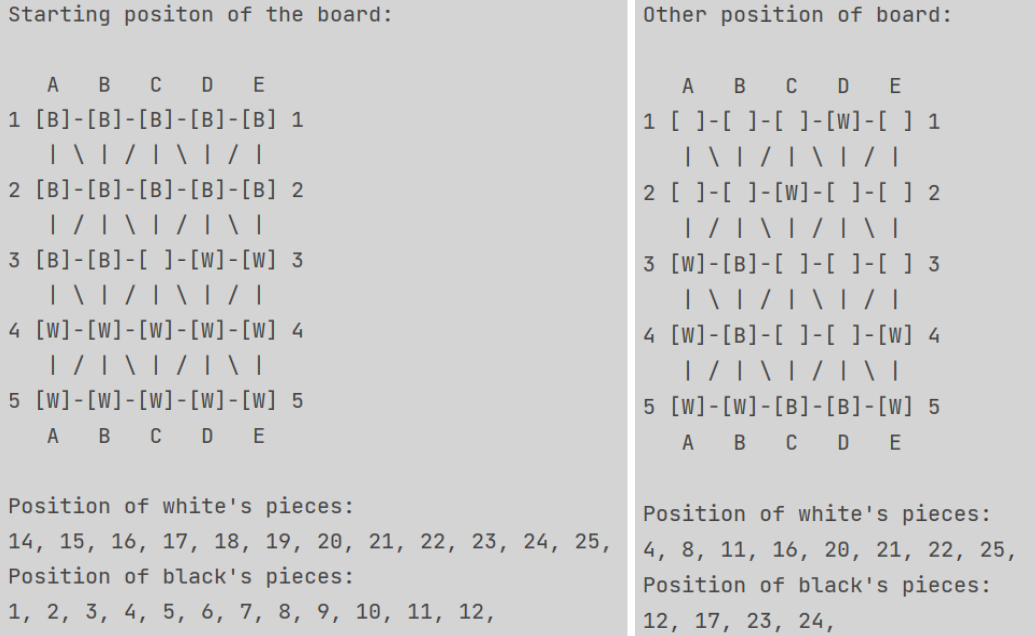
\includegraphics[width=0.9\textwidth]{2in1.png}	
\end{figure}

As seen on picture 1, the starting position for white and black pieces are printed correctly on and below the board.
As seen on picture 2, which is an arbitrary end-of-game position, the positions on the board match the ones printed from the respective arrays.

\newpage

\section{Conclusion}
Through the development and testing of the classes \emph{Board} and \emph{Move}, both separately and coherently, a few issues occured. These issues, as described in the test phase of the report, were eliminated. As a result of resolving these issues, each class then worked properly, as intended, and in accordance with the contract for phase 2. Furthermore, as seen through the test-section, the tests have been conducted with the help of a separate test class, developed for that purpose. Along with this, the classes have been tested with our own version of the Alquerque interface, as well as the precompiled version from phase 2. With a significant level of confidence, it can be concluded that the developed versions of classes \emph{Board} and \emph{Move} will work with all other interfaces developed in accordance with the contract from phase 1 of this project, as well as other interfaces developed in a similar fashion adhering to the documentation for \emph{Board} and \emph{Move}.


\newpage

\section{Appendix}
\subsection{Move class}
\lstinputlisting[style=JavaStyle]{../../src/Move.java}
\newpage
\subsection{Board class}
\lstinputlisting[style=JavaStyle]{../../src/Board.java}
\newpage
\subsection{MainTest}
This was just made for testing purposes and is not expected to run in its current state, since all is uncommented for display purposes, but the individual test segments does work.
\lstinputlisting[style=JavaStyle]{../../src/MainTest.java}
\end{document}
